\section{Experiments and Results}\label{sec:experiments}
Experiments were performed on both stationary and moving datasets.  Our \texttt{stationary} dataset is approximately 22 minutes long and was collected using the Upson Hall antenna on November 11, 2013 starting at approximately 7:39 PM EST.  Weather parameters for the neutral atmosphere corrections were obtained from wunderground.com.  Our moving datasets include those distributed on the course website.  While we evaluated our methods on all datasets, we present in this paper results for \texttt{airportloop} and \texttt{cudtrt13triphammercu}. \texttt{airportloop} offers an interesting case where most of the route is unaffected by multipath errors since tall buildings or overhanging trees are not present.  Additionally, the weather measurements should be quite accurate, assuming they were acquired using the weather station located at the airport.  In contrast, \texttt{cudtrt13triphammercu} offers many challenging examples of line-of-sight occlusion and multipath reflections as well as long stretches of highway for the filter to recover.

We evaluate several versions of our time-varying Kalman filters, each with different turning parameters.  In addition, we also compare to results obtained by using a steady-state Kalman filter built with MATLAB's \texttt{dlqe}, and the two static filters described in~\cite{course}.  Interactive, qualitative results for all datasets can be viewed at \url{http://cs5150.kmatzen.com} until February 2014.

Our first attempt at designing the measurement covariance matrix involved using $\sigma_{PR}$ and $\sigma_D$ from \texttt{solveposvelod}.  In practice, we found two issues with these estimates, both stemming from being estimated by so few satellites at each epoch.  One is that they tend to vary quickly and the other is that they seem to produce filters that were over-confidence in the measurements.  We instead take a moving average of the estimated variances.  Then we tuned the process covariance matrix until the filter passed our consistency test.  For the moving datasets, tuning the process covariance matrix had very little impact on whether or not we could pass the consistency test, presumably due to process mis-modeling.  Instead, we scaled the measurement covariance up by some constant factor for the entire dataset until we could pass the test.

\subsection{Stationary Receiver}
Figure~\ref{fig:stationary_map} shows the estimated position of the receiver's antenna at the end of the dataset sequence.  The consistency test was used to tune the process covariance matrix to $2\times10^-3I$ and the measurement covariance matrix was not rescaled.  

\subsection{Airport Dataset}
Figure~\ref{fig:airportloop_map} shows the estimated trajectory of the vehicle using our time-varying Kalman filter.  This was estimated using a process covariance matrix of $Q = 10I$ and a measurement covariance matrix scaled by $3.5$ in order to pass the consistency test.  This is a very easy dataset, except one set of trees pose a significant challenge for the filter.  The covariance grows quite large until the vehicle passes the trees.  Figure~\ref{fig:airportloop_map_bad} illustrates what happens if we do not scale the measurement covariance matrix to ensure a consistent filter. 

\begin{figure}
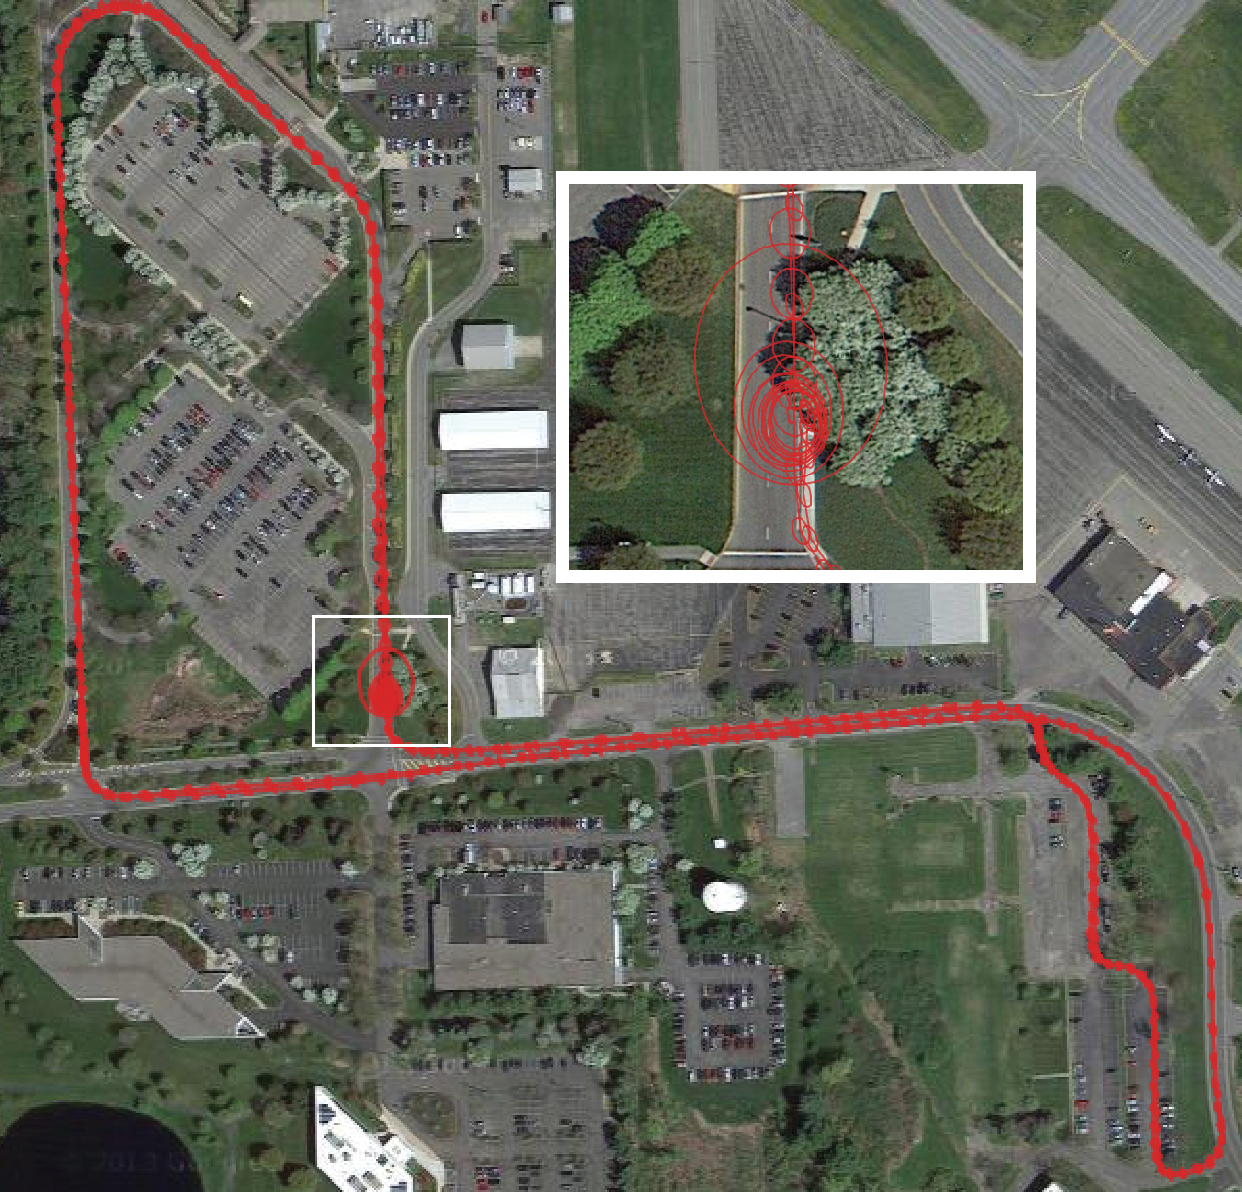
\includegraphics[width=\columnwidth]{airportloop_map}
\caption{Estimated trajectory for \texttt{airportloop} using time-varying Kalman filter adjusted to pass consistency test.  Inset: Highly erroneous navigation solutions lead to an increase in estimation distribution covariance.}
\label{fig:airportloop_map}
\end{figure} 

\begin{figure}
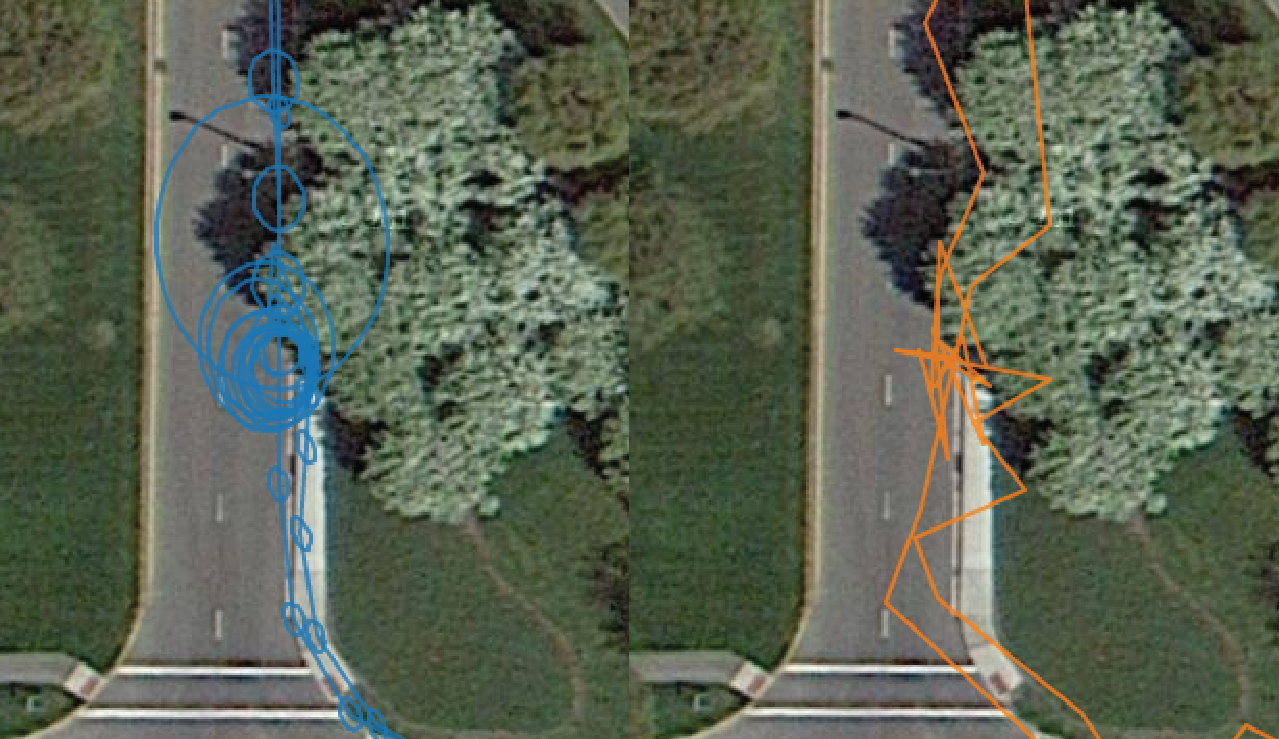
\includegraphics[width=\columnwidth]{airportloop_map_bad}
\caption{Without ensuring filter consistency, the filter can grow over-confident and Kalman filter assumptions that lead to optimality can be broken.  Here, the vehicle is estimated to be on the sidewalk.}
\label{fig:airportloop_map_bad}
\end{figure}
